\documentclass[12pt]{article}

\usepackage{sbc-template}
\usepackage{graphicx,url}
\usepackage{float}
\usepackage[brazil]{babel}   
%\usepackage[latin1]{inputenc}  
\usepackage[utf8]{inputenc}  

\usepackage{xcolor}
% Definindo novas cores
\definecolor{verde}{rgb}{0.25,0.5,0.35}
\definecolor{jpurple}{rgb}{0.5,0,0.35}
% Configurando layout para mostrar codigos Java
\usepackage{listings}


\bibliographystyle{ieeetr}


\lstset{
	language=Java,
	basicstyle=\ttfamily\small, 
	keywordstyle=\color{jpurple}\bfseries,
	stringstyle=\color{red},
	commentstyle=\color{verde},
	morecomment=[s][\color{blue}]{/**}{*/},
	extendedchars=true, 
	showspaces=false, 
	showstringspaces=false, 
	numbers=left,
	numberstyle=\tiny,
	breaklines=true, 
	backgroundcolor=\color{cyan!10}, 
	breakautoindent=true, 
	captionpos=b,
	xleftmargin=0pt,
	tabsize=4
}
\pagestyle{empty}
     
\sloppy
	\title{Sistema de CEP e Rastreamento de Objetos dos Correios  \\ Exercício Computacional I - Sistemas Distribuídos}

\author{Rafael Gonçalves de Oliveira Viana\inst{1} }


\address{Sistemas de Informação -- Universidade Federal do Mato Grosso do Sul
	(UFMS)\\
  	Caixa Postal 79400-000 -- Coxim -- MS -- Brazil
  \email{rafael.viana@aluno.ufms.br}
}

\begin{document} 

\maketitle

     
\begin{resumo} 	
  Este relatório descreve como funciona um \textit{WebService} assim como sua arquitetura, e relata como foi implementado um sistema cliente e um sistema servidor com interface gráfica para busca de CEP e rastreamento de encomendas dos Correios, utilizando Angular 2 e Nodejs.
\end{resumo}



\section{Introdução}

\section{Arquitetura de um WebServece}
Para poder identificar qual arquitetura que um \textit{WebService} deve possuir devemos examinar os pepéis individuais de cada ator no \textit{WebService} e examinar a pilha emergente de protocolo que o \textit{WebService} pretende utiliza.
O mesmo pode ser publicado na intranet ou na Internet, provendo três possiveis formatos de serviços: Provedor de Serviço, Solicitante de Serviço e o Registro de Serviço.

\subsubsection {Provedor de serviço}
Este é o fornecedor do serviço web. O provedor de serviços implementa o serviço e disponibiliza-o na Internet ou intranet.

\subsubsection {Solicitante de Serviço}
Este é um consumidor do serviço web. O solicitante utiliza um serviço da Web existente abrindo uma conexão de rede e enviando uma solicitação XML.

\subsubsection {Registro de serviço}
Este é um diretório de serviços logicamente centralizado. O registro fornece um lugar central onde os desenvolvedores podem publicar novos serviços ou encontrar os existentes. Ele serve como centro de compensação centralizado para empresas e seus serviços.

\subsection{Pilha de protocolo de serviço da Web}
Uma segunda opção para identificar qual arquitetura o  \textit{WebService} deve utiliza é examinar a pilha emergente de protocolo que pretende utilizar. Cada dia existe mais tipos de protocolos porém existem 4 tipo que se destacam: Serviço de Transporte - "FTP", Mensagens "XML", Descrição de Serviço "WSDL"  e Descoberta de Serviço "UDDI" 

\subsubsection {Serviço de transporte}
Esta camada é responsável pelo transporte de mensagens entre aplicativos. Atualmente, esta camada inclui o protocolo de transporte de hipertexto (HTTP), protocolo de transferência de correio simples (SMTP), protocolo de transferência de arquivos (FTP) e protocolos mais recentes, como o protocolo de intercâmbio extensível de blocos (BEEP).

\subsubsection {Mensagens XML}
Esta camada é responsável por codificar mensagens em um formato XML comum para que as mensagens possam ser entendidas em cada uma das extremidades. Atualmente, esta camada inclui XML-RPC e SOAP.

\subsubsection {Descrição do Serviço}
Esta camada é responsável por descrever a interface pública para um serviço web específico. Atualmente, a descrição do serviço é tratada através do Web Service Description Language (WSDL).

\subsubsection {Descoberta do serviço}
Esta camada é responsável por centralizar os serviços em um registro comum e fornecer funcionalidades fáceis de publicação / pesquisa. Atualmente, a descoberta do serviço é tratada através de Descrição Universal, Descoberta e Integração (UDDI).

\subsection {Serviço de Transporte}
A parte inferior da pilha de protocolos do serviço web é o transporte de serviços. Essa camada é responsável por transportar mensagens XML entre dois computadores.

\subsubsection {Hyper Text Transfer Protocol (HTTP)}
Atualmente, o HTTP é a opção mais popular para o transporte de serviços. O HTTP é simples, estável e amplamente implantado. Além disso, a maioria dos firewalls permitem o tráfego HTTP. Isso permite que mensagens XML-RPC ou SOAP se mostrem como mensagens HTTP. Isso é bom se você quiser integrar aplicativos remotos, mas eleva uma série de preocupações de segurança.

\subsubsection {Bloqueia o protocolo de troca extensível (BEEP)}
Esta é uma alternativa promissora para o HTTP. O BEEP é uma nova estrutura da Task Force de Engenharia da Internet (IETF) para a construção de novos protocolos. O BEEP está em camadas diretamente no TCP e inclui uma série de recursos internos, incluindo um protocolo inicial de handshake, autenticação, segurança e tratamento de erros. Usando BEEP, pode-se criar novos protocolos para uma variedade de aplicações, incluindo mensagens instantâneas, transferência de arquivos, distribuição de conteúdo e gerenciamento de rede.

O SOAP não está vinculado a nenhum protocolo de transporte específico. Na verdade, você pode usar SOAP via HTTP, SMTP ou FTP. Uma idéia promissora é, portanto, usar SOAP sobre BEEP.



\section{Componentes de um WebServece}
Ao longo dos últimos anos, três tecnologias primárias emergiram como padrões mundiais que constituem o núcleo da tecnologia de serviços da Web de hoje. Essas tecnologias são demostradas abaixo.

\subsection{XML-RPC}
Este é o protocolo XML mais simples para trocar informações entre computadores.

\begin{enumerate}
	\item XML-RPC é um protocolo simples que usa mensagens XML para executar RPCs.
	\item Os pedidos são codificados em XML e enviados via HTTP POST.
	\item As respostas XML são incorporadas no corpo da resposta HTTP.
	\item O XML-RPC é independente da plataforma.
	\item O XML-RPC permite que diversas aplicações se comuniquem.
	\item Um cliente Java pode falar XML-RPC para um servidor Perl.
	\item XML-RPC é a maneira mais fácil de começar com os serviços da Web.
\end{enumerate}
\subsection{WSDL}
O WSDL é um idioma baseado em XML para descrever os serviços da Web e como acessá-los.

\begin{enumerate}
\item WSDL significa Web Services Description Language.
\item O WSDL foi desenvolvido conjuntamente pela Microsoft e pela IBM.
\item WSDL é um protocolo baseado em XML para troca de informações em ambientes descentralizados e distribuídos.
\item WSDL é o formato padrão para descrever um serviço web.
\item A definição WSDL descreve como acessar um serviço da Web e quais as operações que ele executará.
\item O WSDL é um idioma para descrever como se relacionar com serviços baseados em XML.
\item WSDL é parte integrante do UDDI, um registro de negócios mundial baseado em XML.
\item WSDL é o idioma que UDDI usa.
\item WSDL é pronunciado como "Wiz-Dull" e explicado como 'WSD-L

\end{enumerate}
\subsection{SOAP}
O SOAP é um protocolo baseado em XML para trocar informações entre computadores.

\begin{enumerate}
	\item O SOAP é um protocolo de comunicação.
	\item O SOAP é para comunicação entre aplicativos.
	\item O SOAP é um formato para enviar mensagens.
	\item O SOAP é projetado para se comunicar via Internet.
	\item O SOAP é independente da plataforma.
	\item O SOAP é independente da linguagem.
	\item O SOAP é simples e extensível.
	\item O SOAP permite que você percorra os firewalls.
	\item O SOAP será desenvolvido como um padrão W3C.
\end{enumerate}

\subsection{Exemplo Ilustrativo}
\begin{figure}[H]
	\centering
	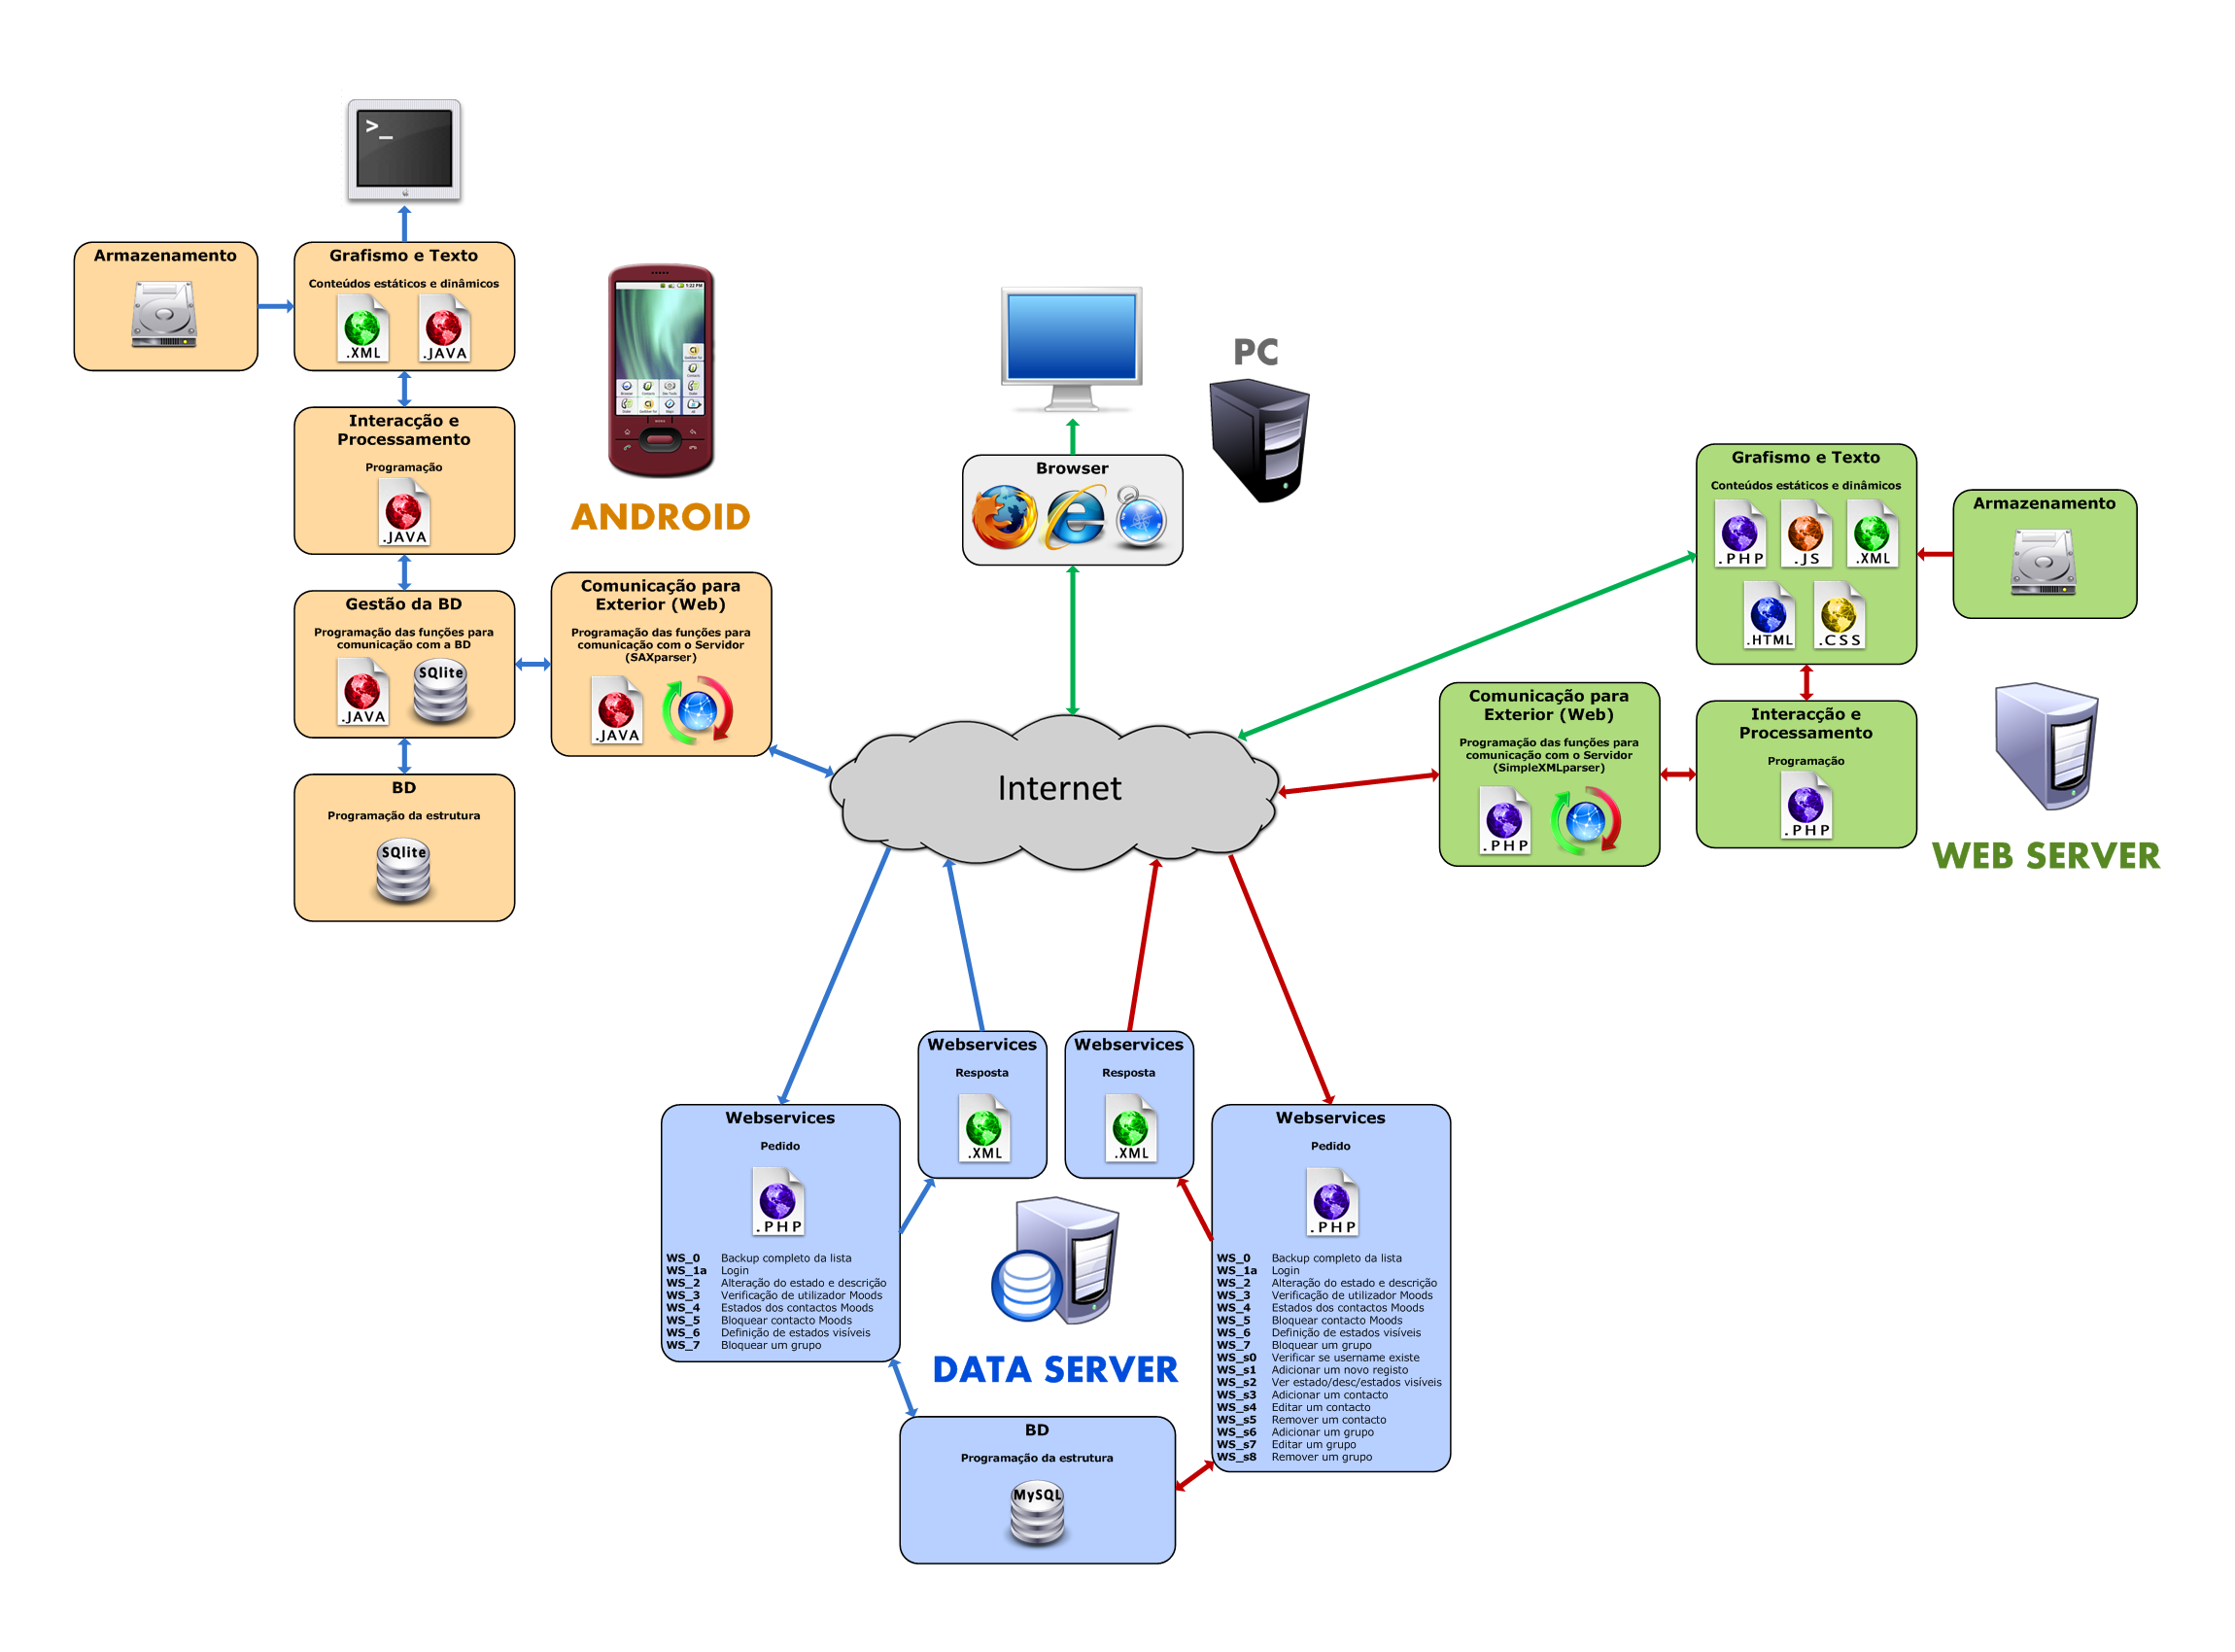
\includegraphics[scale=0.18]{Imagens/webservice.png}
	\caption{Legenda}
	\label{wbs}
\end{figure}
\section{Metodologia}
	\subsection{Tecnologias utilizadas}
	\subsection{Front-End}
	\subsection{Back-end}
	\subsection{Hospedagem}
\section{Conclusão}

 \bibliography{bibli}

\end{document}


